\documentclass[conference]{IEEEtran}
\IEEEoverridecommandlockouts
% The preceding line is only needed to identify funding in the first footnote. If that is unneeded, please comment it out.
\usepackage{cite}
\usepackage{amsmath,amssymb,amsfonts}
%\usepackage{algorithmic}
\usepackage{graphicx}
\usepackage{textcomp}
\usepackage{xcolor}
\usepackage{enumerate}
\usepackage{tabularx}
\usepackage{algorithm}
\usepackage[noend]{algpseudocode}
\newcommand\numberthis{\addtocounter{equation}{1}\tag{\theequation}}
\def\BibTeX{{\rm B\kern-.05em{\sc i\kern-.025em b}\kern-.08em
    T\kern-.1667em\lower.7ex\hbox{E}\kern-.125emX}}
\begin{document}

\title{Container-based Service State Management in
Cloud Computing\\
\thanks{978-3-903176-32-4 ©2021 IFIP}

}

\author{\IEEEauthorblockN{ Shubha Brata Nath , Sourav Kanti Addya , Sandip Chakraborty , Soumya K Ghosh}
\IEEEauthorblockA{\textit{Department of Computer Science and Engineering} \\
Indian Institute of Technology , Kharagpur, India    National Institute of Technology Karnataka, Surathkal, India}
 Email : nath.shubha@gmail.com , souravkaddya@nitk.edu.in , sandipc@cse.iitkgp.ac.in , skg@cse.iitkgp.ac.in


}

\maketitle

\begin{abstract}
Abstract—In a cloud data center, the client requests are catered
by placing the services in its servers. Such services are deployed through a sandboxing platform to ensure proper isolation
among services from different users. Due to the lightweight
nature, containers have become increasingly popular to support
such sandboxing. However, for supporting effective and efficient
data center resource usage with minimum resource footprints,
improving the containers’ consolidation ratio is significant for
the cloud service providers. Towards this end, in this paper,
we propose an exciting direction to significantly boost up the
consolidation ratio of a data-center environment by effectively
managing the containers’ states. We observe that many cloudbased application services are event-triggered, so they remain
inactive unless some external service request comes. We exploit
the fact that the containers remain in an idle state when the
underlying service is not active, and thus such idle containers
can be checkpointed unless an external service request comes.
However, the challenge here is to design an efficient mechanism
such that an idle container can be resumed quickly to prevent
the loss of the application’s quality of service (QoS). We have
implemented the system, and the evaluation is performed in
Amazon Elastic Compute Cloud. The experimental results have
shown that the proposed algorithm can manage the containers’
states, ensuring the increase of consolidation ratio.

\end{abstract}

\begin{IEEEkeywords}
Container, State Management, Service Management, Cloud Computing, Container Migration, Checkpointing
\end{IEEEkeywords}

\section{INTRODUCTION}
Containers [1] have emerged as an essential and effective alternative for hypervisor-based virtualization that complements
the virtual machines (VMs) with a lightweight orchestration
framework while providing an isolated, standalone, and reliable computing environment. Containers [2] can run over baremetals and within a VM, and therefore, it offers significant
computation flexibility for application services deployment.
Due to its low overhead, container-based virtualization supports higher consolidation (number of container-based virtual
servers that can run over a host) compared to hypervisor-based
virtualization [3]. Consequently, it promotes the dense deployment of user applications over a physical host machine [4]–[6].
In a typical virtualized cloud environment, containers are a
good candidate for deploying stateful application servers [7]
like gaming servers, servers providing machine learning toolboxes like optical character recognition, speech processing,
image processing, etc., augmented reality and virtual reality
servers, and so on. These types of server applications have less dependency on the underlying operating system. Therefore,
a containerized version of those application servers can be
hosted on a cloud platform with less overhead. One typical
nature of such application servers is that they get executed
when some external client requests ask for services; otherwise,
they keep running in an idle state. Therefore, the application
server states can be checkpointed, and the server’s resources
can be released temporarily for the best utilization of the
hardware resources [8]. The application service can be resumed from the checkpoint when some external client requests
come. Although such an approach can significantly improve
the hardware utilization and the cloud environment’s energy
efficiency, dynamic checkpointing for stateful containerized
applications has two major challenges.
\begin{enumerate}[i]
\item Different containers need to be checkpointed dynamically when they are idle, and their operations need
to be resumed later from that state with minimum
startup latency. Also, any partially processed data for
the containerized application needs to be stored.
\item During the restoration of a checkpointed service, sufficient hardware resources are not available at the original
physical host, due to the dynamic application workload
for various other services running over the same physical
host. Therefore, there is a need to share the checkpointed
state of the containers between different computing
servers. Moreover, the checkpointed state needs to be
migrated to a new server based on the demand for
resuming the idle container when external client requests
come for that application service.
\end{enumerate}

Therefore, we require to develop a method for dynamic
checkpointing and restoration of containerized stateful application services so that the consolidation ratio increases.Therefore, we require to develop a method for dynamic
checkpointing and restoration of containerized stateful application services so that the consolidation ratio increases.
The consolidation ratio is defined as average number of
virtual instances on each host [9]. In the proposed system,
the virtual instances are containers. Accordingly, in this paper,
we propose a dynamic container checkpointing and service
migration [10], [11] strategy considering the dynamic application demands and workloads of a containerized stateful
service. In order to solve the above-mentioned challenges, we
formulate an optimization problem and propose a checkpoint
based heuristic algorithm to solve the problem of container
deployment. The objective function considers the increase of consolidation ratio. The major contributions of this work are:
\begin{enumerate}[i]
\item The service should go to checkpointed state by freeing
the idle container’s consumed resources when no request
is coming for that service. Other services that need to
serve the clients are deployed dynamically after deallocating the idle containers. However, this management is
challenging as there is a need to deallocate and allocate
containers based on the container state dynamically.
\item  To analyse the system’s performance, we have performed
experiments in Amazon Elastic Compute Cloud (Amazon
EC2) [12]. For this analysis, Amazon EC2 VMs are taken
as the servers. We have considered docker [13] as the
container engine and Checkpoint/Restore In Userspace
(CRIU) [14] as the software to freeze a running container.
Container state management is done by a shared storage
and the docker checkpoint feature. The shared storage is
created using a network file system (NFS) [15].
\item Whenever the current server can not allocate the checkpointed container, the system supports migration of
docker containers by moving the container’s state in a
new server and starting the container there from the
checkpointed state. The experimental results from Amazon EC2 show that the proposed system can increase the
consolidation ratio.
\end{enumerate}

\section{RELATED WORK}

%\subsection{Maintaining the Integrity of the Specifications}

A number of works have focused on various aspects of the
problem of container based service state management in the
recent literature. In [7], the authors have provided a middleware to achieve high availability for cloud applications. The
solution can compensate the limitations of linux containers in
achieving high availability. They are monitoring the containers
that hosts critical components and checkpoint its state. In
case of a failure, the computation is resumed from the most
recent state. The feasibility of their solution is verified using a
case study. The authors in [16] have performed a container
migration service. It is a filesystem-agnostic and vendoragnostic consistent full-system migration service. The work
incorporates CRIU-based memory migration and focuses on
minimizing the migration time. However, no service response
time related analysis is present in this work. In order to do
failure recovery of multi-tier stateful applications, Gomes et
al. [17] have performed an evaluation of checkpoint services
in both virtualized and physical environments. They have
considered the checkpoint in application-level as well as in
system-level. Though analysis of failover time is given, service
response time is not considered. In [18], the authors have proposed elastic provisioning of virtual machines for containers
deployment which takes into account the heterogeneity of containers requirements and computing resources. Their approach
can determine the container deployment on virtual machines
on-demand while optimizing quality of service (QoS) metrics.
It evaluates the container deployment at runtime considering
the QoS metrics. If it achieves an improvement based on the
QoS metrics, a reconfiguration is planned. The authors in
[19] have modeled the micro-service based application (container) deployment problem to minimize total cost considering
\begin{figure}[htbp]
\centerline{\includegraphics[width=0.5\textwidth]{System design}}
\caption{System architecture}
\label{fig}
\end{figure}
server capacity and service delay as the constraints. They
have proposed a communication efficient framework and a
suboptimal algorithm to determine container placement. In
[20], the authors have developed hybrid autoscaling algorithms
and a network scaling algorithm. The hybrid autoscaling
algorithm provides high availability by horizontal scaling and
fine-grained resource control by vertical scaling. The authors
in [21] have solved the problem of container placement across
heterogeneous infrastructure to minimize the overall energy
consumption and balance the load of the hosts. The problem have been formulated as a multi-objective optimization
problem. The authors have solved the problem based on an
incremental exploration of the solution space. The works of
[22] have introduced a resource allocation framework for the
containerized deployment of microservices to reduce operating
costs while providing a minimum guaranteed level of service.
From the above discussion, we observe that the existing
studies mostly look into the placement of the services along
with migration needs. Our objective is to increase the consolidation ratio i.e. increase the number of containers per host.

\section{ SYSTEM ARCHITECTURE}
The proposed architecture of the system is discussed in
this section, which consists of the following components
(Figure 1).
\begin{enumerate}[i]
\item \textbf{Clients}: Clients send service request to the manager
node of the cloud data center.
\item \textbf{Manager Node}: The manager node is connected to all
the worker nodes of the cloud data center. The manager
node has a container allocation and deallocation module
to place the services in the cloud data center. This node
does the aggregation of the results. Also, the final result
is sent to the clients. We need to find the status of the
container state (active/idle). This work is performed by
the state management module. The container allocation

\begin{figure}[htbp]
\centerline{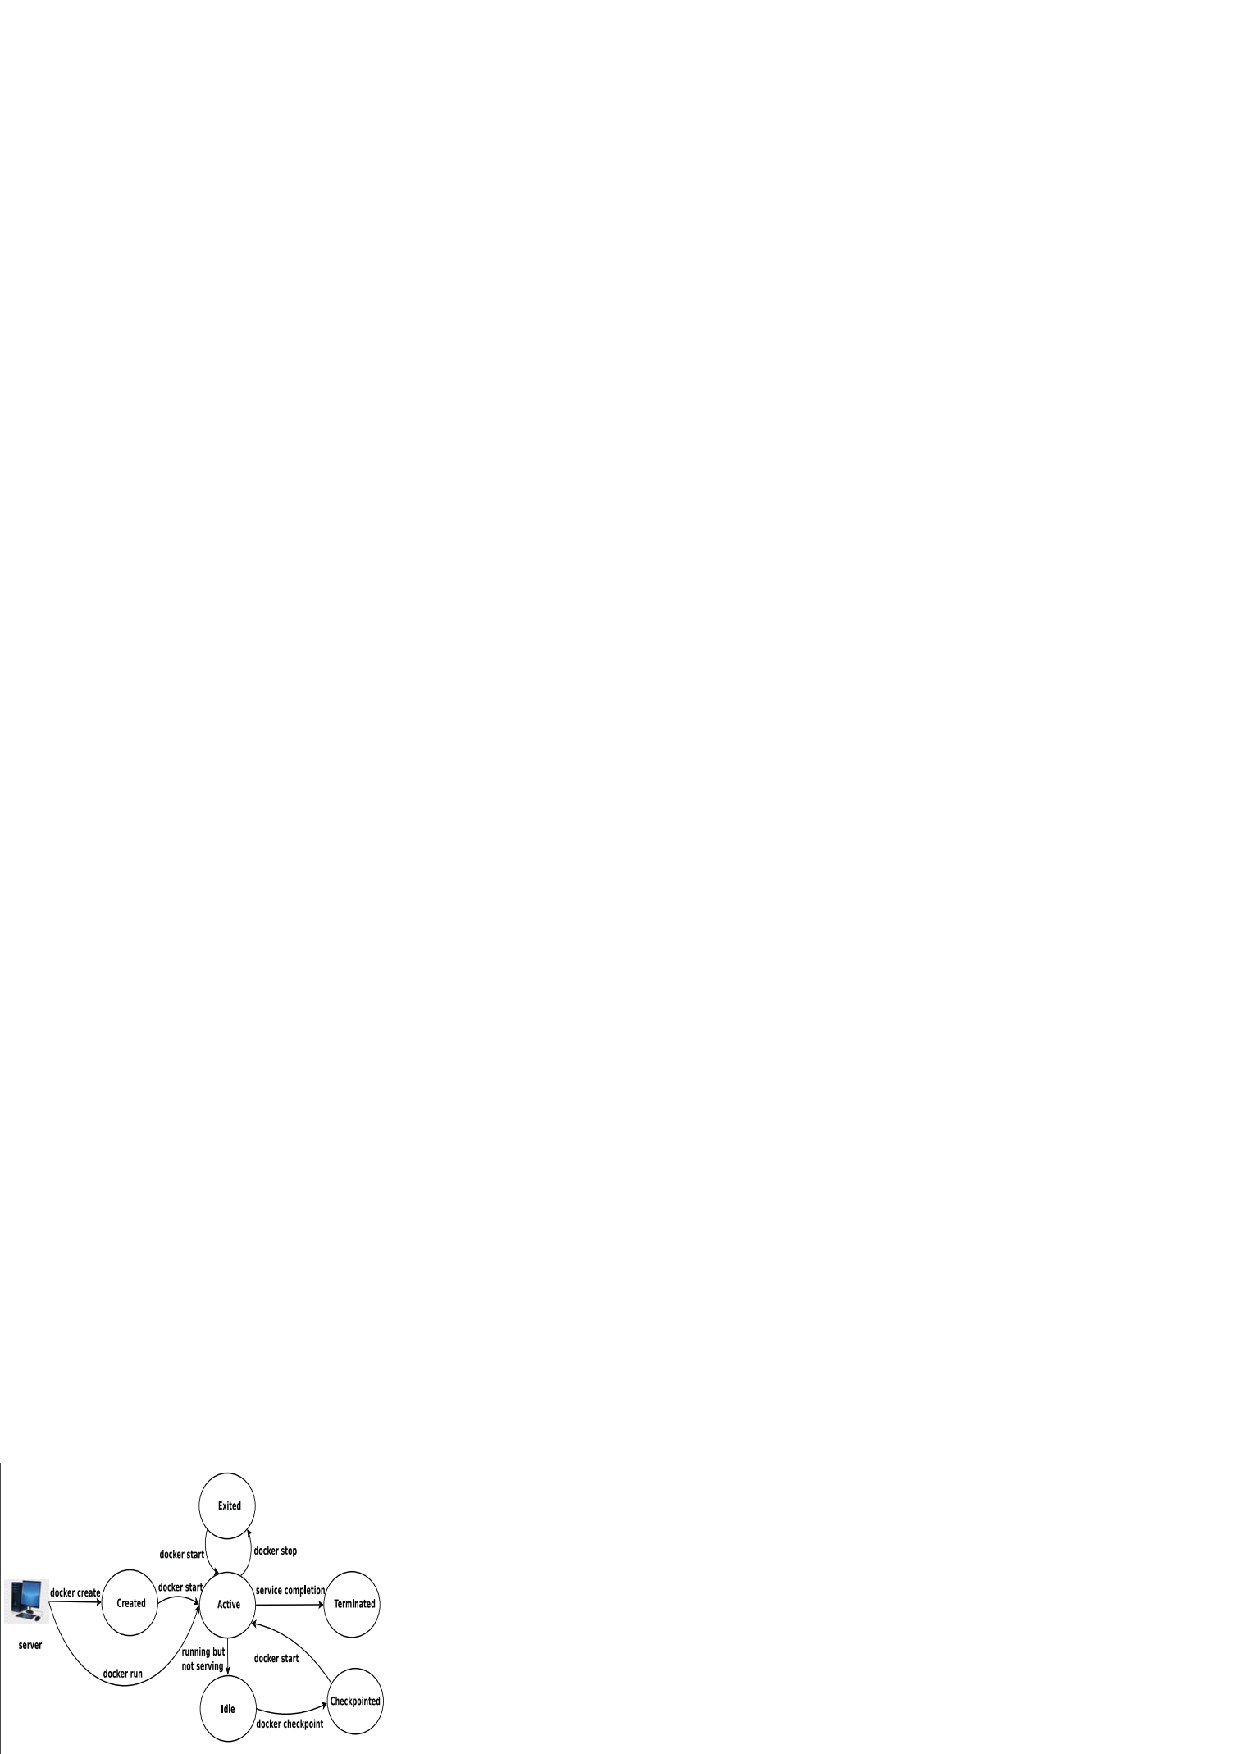
\includegraphics[width=0.5\textwidth]{fig2}}
\caption{ State transition diagram of a docker container}
\label{fig}
\end{figure}
and deallocation module checkpoints the idle containers.
If the current server does not have sufficient resources,
we need to migrate the container to a new worker node.
This migration is performed by the migration manager
module of the manager node. State management module
is responsible for letting the migration manager module
know about the idle containers to be migrated at each
time instant.
\item \textbf{Cloud Worker Node}: The cloud worker node has
container engine (https://docs.docker.com/get-started/
overview/) to run different services as a container.
\item \textbf{Shared Storage using Network File System}: The cloud
worker nodes share a storage to save the state of the
checkpointed containers. This shared storage is designed
using NFS. NFS server is configured in a worker node
that needs to share its directory with other worker nodes.
NFS client is configured in the worker nodes that need
to access the NFS server’s directory.
\end{enumerate}
The management of a container’s states is a very challenging
task as a container goes through many states in its lifecycle. We discuss the state transition of a docker container in
Figure 2. When a docker is running and serving the requests,
it goes to an active state. The docker container goes to an
idle state when it is running but not serving any requests.
Docker containers can be checkpointed to save the current
running state of the container. The docker container goes to
a checkpointed state when we save the running state of the
container. The checkpointed container can be resumed to make
it active again. After the complete service completion, the
docker container goes to a terminated state.

\section{ SERVICE STATE MANAGEMENT OF CONTAINERIZED
APPLICATIONS}
Let us consider c containers and s servers present in the
system at a particular time instant. We denote \begin{math} S = \{ S\textsubscript{i} :   i \in (1,...,s) \} \end{math} and \begin{math} C\textsubscript{i} = \{C\textsubscript{j} : j \in (1,...,c)\}\end{math} as sets of cloud
data center servers and containers respectively.
\subsection{Average Startup Latency of the Services}
We need to start the checkpointed service whenever a
request comes. Therefore, the startup latency for the checkpointed container is defined as
\begin{align*} Startup\_latency\textsubscript{i} = Container\_resumption\_time\textsubscript{i}+
\\ Migration\_time\textsubscript{i}\end{align*}
where \begin{math} Container\_resumption\_time\textsubscript{i}\end{math} is the time taken by
the system to resume the container \begin{math} i \end{math} and \begin{math} Migration\_time\textsubscript{i} \end{math} is the communication time needed to transfer the state from
the source node to the destination node for the container \begin{math}i \end{math}. We define the startup latency for the new container as \begin{align*} Startup\_latency\textsubscript{i} = Container\_deployment\_time\textsubscript{i}\end{align*} where \begin{math} Container\_deployment\_time\textsubscript{i} \end{math} is the time taken by
the system to deploy the new container \begin{math} i \end{math}. \begin{math}Startup\_latency\textsubscript{i} \end{math} is the individual startup delay of a service \begin{math} i \end{math}. Therefore, the
average startup latency is defined as \begin{align*} Avg\textsubscript{startup\_latency} =\frac {\sum_{n=1}^{c} Startup\_latency\textsubscript{i}} {c} \end{align*}

\subsection{Average Response Time of the Services}
We define the response time of a service as
\begin{align*} Resp\_time\textsubscript{i} = Startup\_latency\textsubscript{i}+
 Service\_running\_time\textsubscript{i}\end{align*}
where \begin{math} Service\_running\_time\textsubscript{i}\end{math}
is the processing time taken
for a service in a server. Now, we define the average response
time of the services as,
\begin{align*} Avg\textsubscript{resp\_time} =\frac {\sum_{n=1}^{c} Resp\_time\textsubscript{i}} {c} ,\end{align*}
where \begin{math} Resp\_time\textsubscript{i}\end{math} is the individual response time of a service \begin{math} i \end{math}

\subsection{Constraints}
We define \begin{math} $$C_{j}^{CPU}$$ , $$C_{j}^{RAM}$$ ,  $$C_{j}^{BW}$$\end{math} and \begin{math}  $$C_{j}^{BW}$$\end{math} as the CPU, RAM, and bandwidth resources needed by a container \begin{math} C_j \end{math}
respectively. The available CPU, available RAM, and available bandwidth
of the server \begin{math} S\textsubscript{j}\end{math} are \begin{math}$$Re_{i}^{CPU}$$ , $$Re_{i}^{RAM}$$ ,  $$Re_{i}^{BW}$$ \end{math} respectively. We find \begin{math} k\end{math} servers \begin{math} K = (S\textsubscript{1}.....S\textsubscript{k})\end{math}  from the set of all servers \begin{math} S\end{math} where \begin{math} K \subseteq S\end{math} such that the following conditions are true. 
\begin{align*} \sum_{j=1}^{TC\textsubscript{i}} C_{j}^{CPU} \times x \textsubscript{i,j} \leq Re_{i}^{CPU} \times y\textsubscript{i} \numberthis \label{eqn} \end{align*}
\begin{align*} \sum_{j=1}^{TC\textsubscript{i}} C_{j}^{RAM} \times x \textsubscript{i,j} \leq Re_{i}^{RAM} \times y\textsubscript{i}\numberthis \label{eqn} \end{align*}
\begin{align*} \sum_{j=1}^{TC\textsubscript{i}} C_{j}^{BW} \times x \textsubscript{i,j} \leq Re_{i}^{BW} \times y\textsubscript{i} \numberthis \label{eqn} \end{align*}
where \begin{math} i = 1,....,s\end{math} and \begin{math} 0 \leq j \leq c\end{math}. We define \begin{math} x\textsubscript{i,j}\end{math} as the decision variable to denote if a container \begin{math} C_{j}\end{math} j has been placed in the server \begin{math} S_{j}\end{math}  Also, \begin{math} y_{i}\end{math} is the decision variable to denote if a server \begin{math} S_{i}\end{math} is used for placement or not. TC\textsubscript{i} is the total number of
containers present in the server  \begin{math} S_{i}\end{math}.
\begin{align*} \sum_{i=1}^{S} y\textsubscript{i} \geq 1 \numberthis \label{eqn} \end{align*} 
\begin{align*} \forall_{i,j}  x\textsubscript{i,j} \in \{0 , 1\} ; \forall_{j} y\textsubscript{i} \in \{0 , 1\} \numberthis \label{eqn} \end{align*} 
The following equation states that all the containers should
be deployed in the system. 
\begin{align*} \sum_{i=1}^{k} TC\textsubscript{i} =\mathopen | C \mathclose | \numberthis \label{eqn} \end{align*} 
where \begin{math}\mathopen | C \mathclose | \end{math} is the cardinality of the set \begin{math} C \end{math}.
We have another constraint that one container can be placed
in exactly one server.
\begin{align*}  \forall_{j} \sum_{i=1}^{k} x\textsubscript{i,j} =1 \numberthis \label{eqn} \end{align*} 

\section{ALGORITHM DESIGN}
We propose a heuristic algorithm called Service Deployment
Algorithm to find a near optimal solution. Also, we present
Container Checkpointing Algorithm and Container Resumption Algorithm to checkpoint and resume the containers respectively. We discuss the algorithms below
\subsection{Service Deployment Algorithm}
We present the Service Deployment Algorithm in Algorithm 1. The inputs of the algorithm are container set (C) and
cloud server set (S). The output of the Consolidation ratio.
Our aim is to maximize the consolidation ratio. The checkpointed containers are deployed in the same server where it run
last time if the server is able to meet the resource requirement
(Eq. (1, 2, 3)). Otherwise, a new server is chosen to deploy
the checkpointed container. The proposed algorithm deploys
the containers in the selected server (Su). If the resource
requirement is not met for some containers, we find whether
a checkpoint in the selected server can give enough resources
for the container to be deployed. If a checkpoint can give
the required resources, we identify the idle containers in the selected server and checkpoint them. This approach frees up
more resources that can be allocated to the new containers.
Otherwise, a new server is chosen for checking if deployment
is possible or not. In this way, the consolidation ratio is
maximized by our proposed algorithm. 

\begin{algorithm}
\caption{Service Deployment Procedure}
\begin{algorithmic}[1]
\State \textbf{Input : } Container Set ($C), Cloud Server Set ($S)
\State \textbf{Output : } \begin{math}Consolidation\_ratio \end{math}
\Procedure{Deployment}{$C,S$}       
    \State Sort the containers in descending order of their
resource requirement and store in \begin{math}Sorted\_con\end{math};
\For{$all\ the\ containers\ in\  Sorted\_con$} \begin{math} servers\_not\_available = 0\end{math} \EndFor
    
    \If{$the\ deployment\ request\ is\ for\ a\ checkpointed\
container$} \State \begin{math}k = -1\end{math} 
\State /*\begin{math}S\_last\_run\_C\textsubscript{i}\end{math} is server where the checkpointed container run last time*/
\State \begin{math}S\textsubscript{u} = S\_last run\_C\textsubscript{i};\end{math}
\Else
\State \begin{math}k = 0;\end{math}
\State \begin{math}S\textsubscript{u} = S[k];\end{math}
    \EndIf

    \While{the resource requirement of container C\textsubscript{i}
is greater than  the resource available in
server S\textsubscript{u}} 
         \If{$checkpointing\ in\ server\ S\textsubscript{u}\ can\ deploy\
the\ container\ C\textsubscript{i}$} \State \begin{math}resource\_available\_in\_server =
Checkpoint\_idle\_containers(S\textsubscript{u});\end{math} 
\State Break the while loop

    \EndIf
 \If{$all\ servers\ are\ explored$} \State \begin{math}/*servers\_not\_available\end{math} is set
to 1 if no servers are
found for deployent*/
\State \begin{math}servers\_not\_available = 1\end{math}
\State Break the while loop
\Else
\State  \begin{math}k = k + 1\end{math}
\State \begin{math}S\textsubscript{u} = S[k];\end{math}
    \EndIf
 \If{$servers\_not\_available \neq 1$} \State Deploy the required container C\textsubscript{i} in the selected
server S\textsubscript{u};

\State Calculate \begin{math}Consolidation\_ratio \end{math}
    \EndIf

    \EndWhile  \label{loop}
\State \textbf{return} \begin{math}Consolidation\_ratio \end{math}
\EndProcedure

\end{algorithmic}
\end{algorithm}
\subsection{Container Resumption Algorithm}
In this subsection, we present the Container Resumption
Algorithm for resuming the idle containers. This algorithm
is described in Algorithm 3. The inputs of the algorithm
are the containers that need to be resumed (\begin{math}C\_resume \end{math}), the
container set (\begin{math}C\end{math}), and the cloud server set (\begin{math}S\end{math}). The output of
the algorithm is the \begin{math}Consolidation\_ratio \end{math}.

\section { PERFORMANCE EVALUATION}
We performed the experiments in Amazon EC2 (https://aws.
amazon.com/ec2/) using python 2.7.13.
\subsection {Implementation Details}
The cloud servers have Ubuntu 18.04 long-term support
(LTS) (https://www.ubuntu.com/) operating system. Also, we
use Docker [24] as the container engine in the servers. The
docker version taken for the implementation is 17.03.2-ce.
To perform the docker checkpoint, the docker experimental
feature is enabled and CRIU (https://criu.org/Main Page) is
installed in the servers. Docker uses CRIU [25] to manage the
lifecycle of processes running inside its containers (https://criu.
org/Docker). We set up the shared storage using NFS (https://help.ubuntu.com/lts/serverguide/network-file-system.html) to
make the checkpointed files available in different servers. We
have taken zookeeper application (https://zookeeper.apache.
org/), PHP web application (https://www.php.net/) and redis
application (https://redis.io/) for evaluation. We have analysed
the output of the docker stats command to check the resource
status of a container. We show the values of the parameters
taken in Amazon EC2 experiments in Table I. The topology
considered for these experiments is shown in Figure 3.
\begin{table}[htbp]
\caption{PARAMETERS IN AMAZON EC2 EXPERIMENT}
\begin{center}
\begin{tabularx}{0.4\textwidth} { 
  | >{\raggedright\arraybackslash}X 
  | >{\centering\arraybackslash}X 
  | >{\raggedleft\arraybackslash}X | }
 \hline
 \textbf{Parameter} & \textbf{Value}  \\
 \hline
 Number of Amazon EC2 virtual
machine instances or worker nodes  & 10    \\
\hline
Processor of a worker node & 2.5 GHz Intel Xeon Family \\ 
\hline 
Number of vCPU in a worker node & 1 \\ 
\hline 
Storage of a worker node & 8 GB \\
\hline 
Operating System used & Ubuntu Server 18.04 LTS \\
\hline
Maximum available RAM of the
worker node & 680 MB \\
\hline
Maximum available RAM of the
manager node & 1780 MB \\
\hline
\end{tabularx}
\label{tab1}
\end{center}
\end{table}
\subsection{Competing Heuristics}
We consider Execution Container Placement and Task assignment Algorithm (EPTA) [19] as a baseline. In EPTA,
the microservice controller queries a small local region for
available physical resources. The execution containers are
placed in the server, which has less node cost as well as
less link cost. The microservice controller requests physical
resources and waits for responses from the physical machines
(PM). Once the request is approved, an execution container
is built on the selected PM. If the request is rejected, the
PM is marked as infeasible. When some tasks have not been
successfully assigned, the microservice controller queries PMs
on a larger scale. We have taken first fit decreasing (FFD) as
another baseline. FFD is used in many works in the existing
literature [26], and it is a well-known heuristic for bin packing
problem. In FFD, the containers are sorted in decreasing order
of the size of the required resource. Then, FFD chooses the
first server that is large enough to place the containers.

\section{CONCLUSION}
We have performed the container-based service state management to maximize the cloud data center’s consolidation ratio. In our proposed approach, the idle containers need to
be checkpointed to save the hardware resources. However,
after the end of the idle period, the containers need to be
resumed from the last saved state. The idle containers are
migrated to a new server if the current server does not have
sufficient resources to run it. The problem of state management
of the containers is formulated as an optimization problem that
maximizes the consolidation ratio as the objective function. We
have proposed a heuristic algorithm to solve the optimization.
In order to save the state of an idle container, we have proposed
a container checkpointing algorithm. Also, an algorithm is
proposed for the resumption of idle containers when a request
comes for these services. The evaluation in Amazon EC2
shows that the proposed algorithm is able to maximize the
consolidation ratio ensuring the state management of the containers. Thus, the proposed algorithm can efficiently manage
the service state.

\begin{thebibliography}{00}
\bibitem{b1}  E. Casalicchio, “Container orchestration: A survey,” in Systems Modeling: Methodologies and Tools. Springer, 2019, pp. 221–235.
\bibitem{b2} F. Rossi, V. Cardellini, and F. L. Presti, “Elastic deployment of software
containers in geo-distributed computing environments,” in Proc. of IEEE
ISCC’19, 2019.
\bibitem{b3}  K. Suo, Y. Zhao, W. Chen, and J. Rao, “An analysis and empirical
study of container networks,” in proceedings of the IEEE Conference
on Computer Communications. IEEE, 2018, pp. 189–197.
\bibitem{b4}  A. Celesti, D. Mulfari, M. Fazio, M. Villari, and A. Puliafito, “Exploring
container virtualization in iot clouds,” in 2016 IEEE International Conference on Smart Computing (SMARTCOMP). IEEE, 2016, pp.1–6.
\bibitem{b5}  A. Celesti, D. Mulfari, A. Galletta, M. Fazio, L. Carnevale, and
M. Villari, “A study on container virtualization for guarantee quality
of service in cloud-of-things,” Future Generation Computer Systems,
vol. 99, pp. 356–364, 2019.
\bibitem{b6}  I. M. A. Jawarneh, P. Bellavista, L. Foschini, G. Martuscelli, R. Montanari, A. Palopoli, and F. Bosi, “Qos and performance metrics for
container-based virtualization in cloud environments,” in Proceedings
of the 20th International Conference on Distributed Computing and
Networking. ACM, 2019, pp. 178–182.
\bibitem{b7}  W. Li, A. Kanso, and A. Gherbi, “Leveraging linux containers to
achieve high availability for cloud services,” in 2015 IEEE International
Conference on Cloud Engineering. IEEE, 2015, pp. 76–83.
\bibitem{b8} D. R. Sangolli, N. M. Ravindrarao, P. C. Patil, T. Palissery, and K. Liu,
“Enabling high availability edge computing platform,” in 2019 7th IEEE
International Conference on Mobile Cloud Computing, Services, and
Engineering (MobileCloud). IEEE, 2019, pp. 85–92.
\bibitem{b9} O. Sukwong, A. Sangpetch, and H. S. Kim, “Sageshift: managing slas
for highly consolidated cloud,” in 2012 Proceedings IEEE INFOCOM.
IEEE, 2012, pp. 208–216
\bibitem{b10} W. Fan, Z. Han, P. Li, J. Zhou, J. Fan, and R. Wang, “A live migration
algorithm for containers based on resource locality,” Journal of Signal
Processing Systems, vol. 91, no. 10, pp. 1077–1089, 2019.
\bibitem{b11}  S. Noor, B. Koehler, A. Steenson, J. Caballero, D. Ellenberger, and
L. Heilman, “Iotdoc: A docker-container based architecture of iotenabled cloud system,” in 3rd IEEE/ACIS International Conference on
Big Data, Cloud Computing, and Data Science Engineering. Springer,
2019, pp. 51–68.
\bibitem{b12} S. Yang, L. Pan, and S. Liu, “An online algorithm for selling your
reserved iaas instances in amazon ec2 marketplace,” in 2019 IEEE
International Conference on Web Services (ICWS). IEEE, 2019, pp.
296–303.
\bibitem{b13}  D. N. Jha, S. Garg, P. P. Jayaraman, R. Buyya, Z. Li, and R. Ranjan, “A
holistic evaluation of docker containers for interfering microservices,”
in 2018 IEEE International Conference on Services Computing (SCC).
IEEE, 2018, pp. 33–40.
\bibitem{b14} S. Pickartz, N. Eiling, S. Lankes, L. Razik, and A. Monti, “Migrating
linux containers using criu,” in International Conference on High
Performance Computing. Springer, 2016, pp. 674–684.
\end{thebibliography}


\end{document}
